% Section 6 — L3 Temporal Confabulation (compressed for best-paper density)

\section{The Narrative Axis: Closure, Ceiling, and Catastrophe}
\label{sec:l3}

Section~\ref{sec:l2} showed capability scaling does not help the action axis. This section is its counterpoint: on the narrative axis $\confab := \log_{10}(\tself/\twall)$, capability scaling helps monotonically across five frontier non-reasoning generations ($|\confab|$ from $+1.12$ to $+0.07$, a $94\%$ reduction; full table in App.~\ref{app:full-panel-tables}). The closure is real; it is also bounded in three directions, each with its own \S: a theorem that reasoning-token expansion \emph{reverses} the trend (\S\ref{ssec:reverse-scaling}), a calibration catastrophe that persists even where the surface appears closed (\S\ref{ssec:calibration}), and a constructive positive control that shows what training would actually close it (\S\ref{ssec:a1-positive-control}).

\subsection{The Reverse-Scaling Theorem}
\label{ssec:reverse-scaling}

\paragraph{Assumption (budget-honoured reasoning).}
\label{ass:budget-honoured}
A reasoning-budget knob $K$ on a fixed agent is \emph{honoured} if $\mathbb{E}[\twall \mid K]$ is strictly increasing in $K$. The o4-mini \texttt{reasoning\_effort} ladder, Anthropic extended-thinking budget, and Kimi/GLM reasoning modes all satisfy this empirically. Budgets the model declines to spend (E5 on DeepSeek-R1-Distill-14B, App.~\ref{app:l3-detail}) fall outside the assumption and are not counter-examples.

\begin{theorem}[Reverse-Scaling]
\label{thm:reverse-scaling}
For a fixed agent under Assumption~\ref{ass:token-only} (hence Observation~\ref{thm:cit}) with a budget-honoured $K$, $\mathbb{E}[|\confab| \mid K]$ is monotone non-decreasing in $K$.
\end{theorem}

\begin{proof}[Sketch]
Under CIT, $p(\tself)$ is invariant to $\twall$: no gradient signal ties one to the other. The inference-time distribution $p(\tself \mid K) = p(\tself)$ for all $K$. By assumption, $\twall(K)$ is strictly increasing. Therefore $|\log_{10}(\tself/\twall)|$ is monotone non-decreasing in $K$ in expectation. The sign of $\confab$ turns negative once hidden CoT comes to dominate $\twall$, because $p(\tself)$ stays anchored to the surface output; the theorem itself constrains only $|\confab|$.
\end{proof}

\begin{figure}[h]
\centering
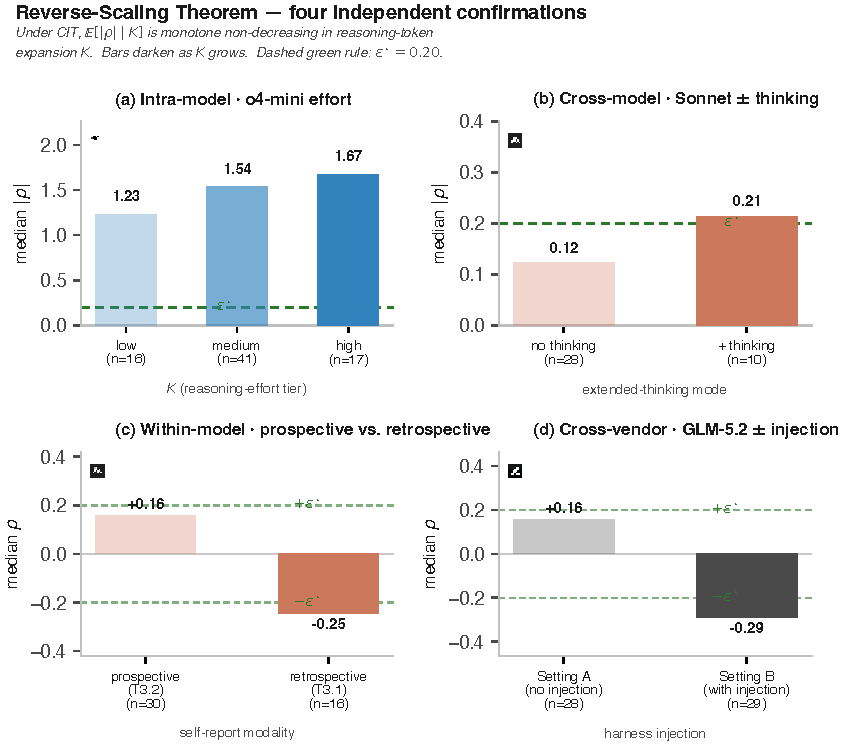
\includegraphics[width=\linewidth]{figures/reverse_scaling.pdf}
\caption{Four independent confirmations of Theorem~\ref{thm:reverse-scaling}. \textbf{(a)} Intra-model: o4-mini \texttt{reasoning\_effort} ladder, $|\confab| = 1.23 \to 1.54 \to 1.67$. \textbf{(b)} Cross-model: Sonnet 4.6 $\pm$ extended thinking, median $|\confab| = 0.12 \to 0.21$ (Setting~A, $n = 28/10$; signed median $+0.07 \to -0.17$), with the sign flip firm under Setting~B ($-0.25$, CI $[-0.34, -0.11]$, $n = 16$). \textbf{(c)} Within-model: Sonnet-thinking prospective ($+0.16$) vs.\ retrospective ($-0.25$) under Setting~B --- sign flip on the same tasks. \textbf{(d)} Cross-vendor: GLM-5.2 (Z.AI, no shared training pipeline with Anthropic), Setting~A $\to$ B: $+0.16 \to -0.29$. Detailed per-cell CIs in App.~\ref{app:full-panel-tables} Tables~\ref{tab:full-panel}--\ref{tab:reasoning-t3}.}
\label{fig:reverse-scaling}
\end{figure}

The four confirmations vary four independent things: reasoning effort within one model, the presence of a thinking mode across two builds of one model, the narration modality within one configuration, and the training pipeline across two vendors that share none of it. All four show the same object --- raising the reasoning budget, or triggering reasoning-mode CoT, grows $|\confab|$. Three of the four also flip its sign toward Hidden-Time under-report, and on Setting~B the three Chinese-lab reasoning models (GLM-5.2, Kimi-K2.6, Qwen3.6-27B) sit collectively at median $\rho \in [-0.97, -0.29]$, which makes the flip a property of the class rather than of Sonnet-thinking.

It is not universal, and we say so: o3 grows $|\confab|$ to $0.45$ --- well above base Sonnet 4.6's $0.12$ on the same tasks --- while continuing to over-report (App.~\ref{app:full-panel-tables}). Theorem~\ref{thm:reverse-scaling} constrains the magnitude, and every cell confirms the magnitude. The sign flip is the mechanism's most visible symptom, not its definition: it appears when the hidden chain-of-thought comes to dominate $\twall$, and o3 is the configuration where it does not.

\subsection{Who Declines to Answer}
\label{ssec:refusal}

The panel tables report an effective $n_\rho$ ``after parser drops''. That
single number turns out to cover four behaviours which mean different things,
and separating them changes how two of our own results should be read.
Classifying all $900$ T3.1 trajectories (App.~\ref{app:l3-detail}): $626$ state
a positive duration and are scored; of the $274$ that are not, $110$ ($40\%$)
are an \emph{explicit refusal} to estimate, $132$ ($48\%$) never mention
duration, $18$ ($7\%$) state a duration of exactly zero, and $14$ ($5\%$) are
positive durations our scorer missed.

\paragraph{Reasoning-mode agents refuse an order of magnitude more often.}
Refusals are not spread evenly. Pooled over settings, reasoning-mode
configurations decline on $21.9\%$ of trajectories ($n = 480$) against $1.2\%$
for non-reasoning ($n = 420$) --- an $18\times$ gap. Sonnet 4.6 $+$ thinking
declines on $57\%$, Kimi-K2.6 on $42\%$, gpt-5.1 on $35\%$, while gpt-4o,
gpt-4o-mini, Haiku 4.5, Qwen2.5-7B and Qwen3.6-27B never once decline. This is
the same object as the cross-lingual refusal asymmetry of
\S\ref{sec:limitations}, seen on the narrative axis instead of the wall axis:
declining to estimate is a surface disposition of post-training, distributed
very unevenly across configurations, and not a representation of the
underlying absence.

\paragraph{Two consequences we report rather than absorb.}
First, $\rho$ for the high-refusal agents is computed on a \emph{selected}
subsample --- the trajectories where the agent chose to commit a number.
Sonnet 4.6 $+$ thinking's $n_\rho = 10$ under Setting~A is not a parsing
failure but a $57\%$ refusal rate, and its contribution to the cross-model
sign flip (Fig.~\ref{fig:reverse-scaling}b) therefore rests on the $43\%$ where
it answered. We cannot bound the direction of that selection from these data;
the intra-model effort ladder and the cross-vendor comparison, whose agents
refuse at $13\%$ and $5\%$, do not carry the same exposure, and the theorem's
magnitude claim is confirmed on all of them.

Second, the $18$ trajectories reporting \emph{exactly zero} seconds are
excluded by the arithmetic rather than by choice: $\rho = \log_{10}(0/\twall)$
is undefined. These are the most extreme under-reports the instrument can
produce, so every $|\confab|$ we report is, by that much, an underestimate. The
bias runs against our own claim, which is the direction we would rather it ran,
but it should be stated.

\subsection{The Calibration Catastrophe}
\label{ssec:calibration}

Asked to wrap self-duration in a $90\%$ confidence interval, every non-reasoning panel agent achieves under-coverage of at least $40$ percentage points (Fig.~\ref{fig:calibration-catastrophe}); GPT-4o reaches $0\%$. Standard post-training calibration tooling (temperature scaling, isotonic regression, RLHF-with-confidence \citep{guo2017calibration,jiang2021calibration,kadavath2022knowing,dontthinktwice2025}) cannot apply, because the calibration signal is not in the loss support (CIT). Pre-registered P11: no CIT-regime agent achieves $> 0.5$ coverage without harness-side duration data.

\begin{figure}[h]
\centering
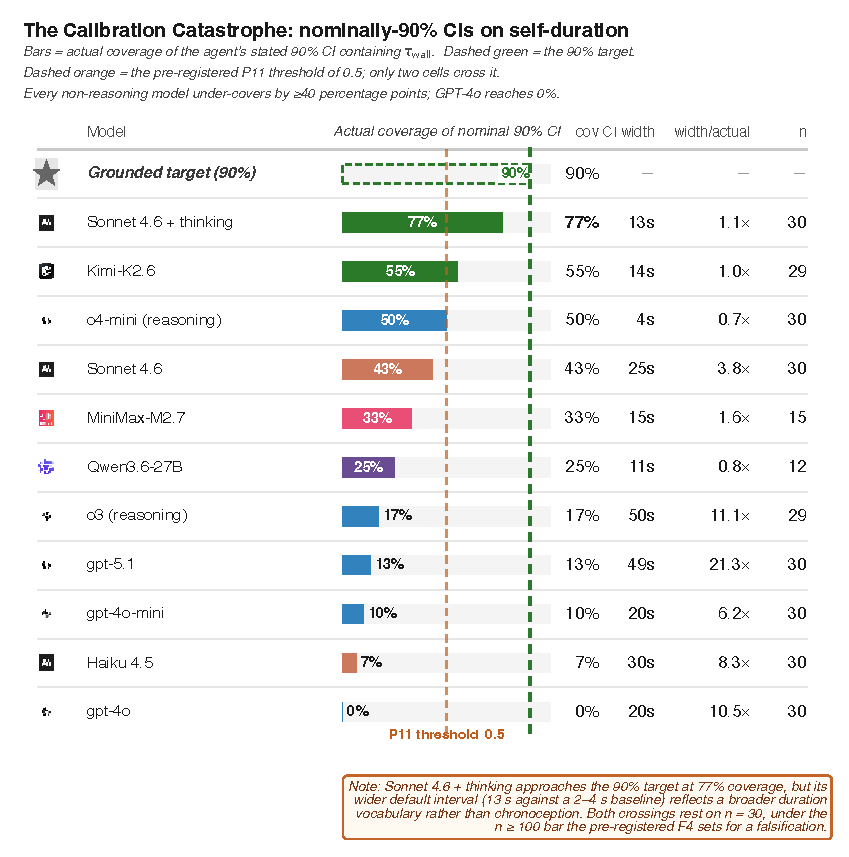
\includegraphics[width=\linewidth]{figures/calibration_catastrophe.pdf}
\caption{Actual coverage of nominally-$90\%$ CIs on self-duration (T3.3), 12-row panel. Only reasoning-mode agents (Sonnet + thinking, Kimi-K2.6) exceed the P11 threshold of $0.5$ --- both accidentally, through wider default vocabulary intersecting thinking-inflated $\twall$ (see App.~\ref{app:l3-detail}), not through learned chronoception.}
\label{fig:calibration-catastrophe}
\end{figure}

\paragraph{Two P11 crossings, one mechanism.}
Two cells cross $0.5$: Sonnet-thinking ($77\%$, $n = 30$, Wilson CI $[0.59, 0.88]$) and Kimi-K2.6 ($55\%$, $n = 29$, Wilson CI $[0.38, 0.71]$). o4-mini lands exactly on the threshold at $15/30$ and so does not cross it. All three are reasoning-mode; all three state intervals far wider relative to their own $\twall$ than the non-reasoning panel does; and Kimi shares no training pipeline with the other two. Two further rows, MiniMax-M2.7 ($n = 15$) and Qwen3.6-27B ($n = 12$), rest on fewer than half the intended trajectories after parser drops and are plotted with their true $n$. The mechanism is not learned chronoception but arithmetic: reasoning-mode inflates $\twall$, $p(\tself)$ stays anchored to the default duration vocabulary, and a wider stated CI happens to contain the wall-clock. Consistent with CIT. Both cells rest on $n = 30$, below the $n \geq 100$ bar our pre-registered F4 sets for a falsification of P11, so we report them as threshold crossings rather than refutations --- but we do report them. They sharpen P11: the next revision should measure a proper scoring rule (Brier / CRPS) rather than raw coverage.

% Section 6.3 --- Positive control (compressed)

\subsection{A positive control: wall-clock SFT installs partial chronoception}
\label{ssec:a1-positive-control}

CIT is a negative result. Can a procedure that includes wall-clock signal install chronoception? We provide a toy positive control.

\paragraph{Construction.}
Qwen2.5-1.5B and 7B base models. For each, 500 SFT pairs of the form ``\textit{\{response\}. This task took approximately \{$\twall$\} seconds.}'' with $\pm 15\%$ noise; LoRA rank $16$, three epochs. Token-level CE loss, but training targets carry $\twall$: the effective loss support includes wall-clock duration, exiting the CIT regime by extending $\mathcal{D}$'s support rather than changing $\ell$.

\paragraph{Result.}
On 30 held-out T3.1 instances: median $|\confab|$ falls from $1.37$ to $0.30$ on 1.5B ($78\%$ reduction) and $0.93$ to $0.50$ on 7B ($46\%$). The 1.5B fine-tuned T3.1 score ($0.151$) crosses $\ccestar$ on this single axis; the 7B ($0.252$) does not (Fig.~\ref{fig:a1-positive}). At both scales $\confab$ flips from over-report to under-report.

\begin{figure}[h]
\centering
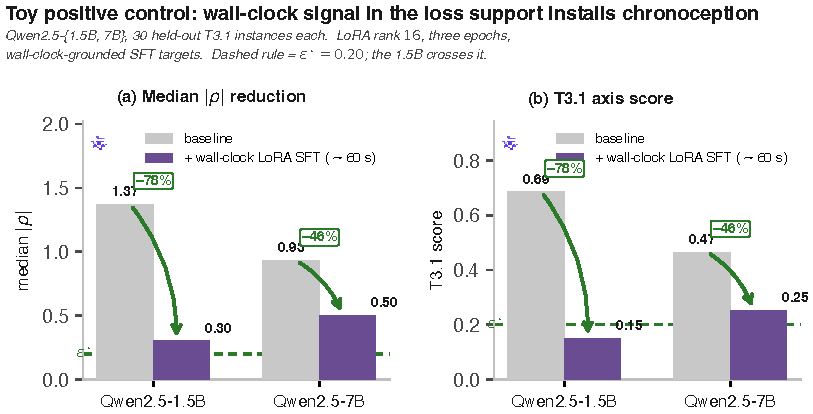
\includegraphics[width=\linewidth]{figures/a1_positive_control.pdf}
\caption{Toy positive control. \textbf{(a)} $|\confab|$ falls at both scales after $\sim$60\,s of LoRA SFT. \textbf{(b)} 1.5B fine-tuned crosses $\ccestar$ on T3.1; 7B partial ($0.25$). Detailed table in App.~\ref{app:l3-detail}.}
\label{fig:a1-positive}
\end{figure}

\paragraph{What it shows and does not show.}
Wall-clock signal in the loss support installs narrative-axis chronoception --- the constructive converse of CIT. The control does not address L2 (which needs the policy to elongate action sequences, not append duration strings) or T3.3 calibration. Full-axis installation is the programme of \textsc{ChronoStack}: action-axis grounding requires a wall-clock-supported reward, calibration requires a conditional-variance objective, full grounding requires architectural support.


The three faces of L3 (Reverse-Scaling, Calibration Catastrophe, positive control) form one picture: narrative training closes the surface for non-reasoning agents; reasoning-token expansion structurally re-opens it; wall-clock support in the loss actually closes it. Narrative axis training does not reach the action axis; the next section shows how the industry has compensated.
